%=====================================================================
\chapter{Resultados}\label{results}
%==================================================================

Neste capítulo serão apresentados alguns dos resultados obtidos para os diversos testes realizados durante a execução desse projeto. Inicialmente serão apresentados valores numéricos e avaliadas as diferenças entre algoritmos adotados, na sequência serão ilustrados os resultados sobre pares de imagens para a conferência visual das correlações e finalmente serão consideradas as variações que podem ser obtidas pela manipulação dos argumentos admitidos na solução construída. 

\section{Resultados numéricos dos testes}

Após codificação do produto final e execução dos testes planejados temos resultados divididos entre subprocessos de imagens, que realiza detecção e descrição de feições; de pares de imagens, que implicam nas correlações e verificações geométricas; e de medidas, que implicam em sumarizar os pontos de costura obtidos.

\subsection{Custo de detecção e descrição}

A apresentação dos resultados foi realizada através da Tabela \ref{Det&Dec} por imagem e, para maior clareza, foram agrupados para cada algoritmo seus tempos de detecção de feições, número de respostas obtidas, uma razão entre esses valores e o espaço de memória alocado em MB (\textit{Mega Byte}) para a resposta. Também foram integrados dados de tempo da descrição de feições e uma razão entre este e o número de feições, além do espaço necessário para manter a descrição disponível para as etapas seguintes no fluxo da aplicação. A última coluna da mesma tabela apresenta médias dos valores anteriores de cada imagem para auxílio na análise.

\begin{table}[!ht]{15,5cm}
\caption{Resultados numéricos de detecção e descrição dos métodos analisados.}\label{Det&Dec}
\begin{tabular}{c|c|c|ccc|c}
\hline
\multirow{2}{*}{Método} & \multirow{2}{*}{Etapa} & \multirow{2}{*}{Medida} & \multicolumn{3}{c|}{Imagens} & \multirow{2}{*}{Média} \\ \cline{4-6}
 &  &  & \multicolumn{1}{c|}{16} & \multicolumn{1}{c|}{17} & 18 &  \\ \specialrule{.1em}{.05em}{.05em}
\multirow{7}{*}{AKaze} & \multirow{4}{*}{Detecção} & Número   de pontos & \multicolumn{1}{c|}{81652} & \multicolumn{1}{c|}{78797} & 73851 & 78100 \\ \cline{3-7} 
 &  & Tempo total   (ms) & \multicolumn{1}{c|}{1208,4} & \multicolumn{1}{c|}{974,291} & 899,603 & 1027,431 \\ \cline{3-7} 
 &  & Tempo / Ponto & \multicolumn{1}{c|}{0,015} & \multicolumn{1}{c|}{0,012} & 0,012 & 0,013 \\ \cline{3-7} 
 &  & Tamanho alocado(MB) & \multicolumn{1}{c|}{2,170} & \multicolumn{1}{c|}{2,100} & 1,970 & 2,080 \\ \cline{2-7} 
 & \multirow{3}{*}{Descrição} & Tempo total (ms) & \multicolumn{1}{c|}{1138,68} & \multicolumn{1}{c|}{1029,09} & 967,404 & 1045,058 \\ \cline{3-7} 
 &  & Tempo / Ponto & \multicolumn{1}{c|}{0,014} & \multicolumn{1}{c|}{0,013} & 0,013 & 0,013 \\ \cline{3-7} 
 &  & Tamanho alocado(MB) & \multicolumn{1}{c|}{19,000} & \multicolumn{1}{c|}{18,330} & 17,180 & 18,170 \\ \specialrule{.1em}{.05em}{.05em} %\hline
\multirow{7}{*}{ORB} & \multirow{4}{*}{Detecção} & Número de   pontos & \multicolumn{1}{c|}{100000} & \multicolumn{1}{c|}{100000} & 100000 & 100000 \\ \cline{3-7} 
 &  & Tempo total   (ms) & \multicolumn{1}{c|}{302,914} & \multicolumn{1}{c|}{261,936} & 267,354 & 277,401 \\ \cline{3-7} 
 &  & Tempo / Ponto & \multicolumn{1}{c|}{0,003} & \multicolumn{1}{c|}{0,003} & 0,003 & 0,003 \\ \cline{3-7} 
 &  & Tamanho alocado(MB) & \multicolumn{1}{c|}{2,660} & \multicolumn{1}{c|}{2,660} & 2,660 & 2,660 \\ \cline{2-7} 
 & \multirow{3}{*}{Descrição} & Tempo total (ms) & \multicolumn{1}{c|}{192,903} & \multicolumn{1}{c|}{203,595} & 190,662 & 195,72 \\ \cline{3-7} 
 &  & Tempo / Ponto & \multicolumn{1}{c|}{0,0019} & \multicolumn{1}{c|}{0,0020} & 0,0019 & 0,002 \\ \cline{3-7} 
 &  & Tamanho alocado(MB) & \multicolumn{1}{c|}{12,2} & \multicolumn{1}{c|}{12,2} & 12,2 & 12,2 \\ \specialrule{.1em}{.05em}{.05em} %\hline
\multirow{7}{*}{SIFT} & \multirow{4}{*}{Detecção} & Número de   pontos & \multicolumn{1}{c|}{114684} & \multicolumn{1}{c|}{106728} & 103486 & 108299 \\ \cline{3-7} 
 &  & Tempo total   (ms) & \multicolumn{1}{c|}{2252,18} & \multicolumn{1}{c|}{1823,36} & 1589,33 & 1888,29 \\ \cline{3-7} 
 &  & Tempo / Ponto & \multicolumn{1}{c|}{0,02} & \multicolumn{1}{c|}{0,017} & 0,015 & 0,017 \\ \cline{3-7} 
 &  & Tamanho alocado(MB) & \multicolumn{1}{c|}{3,06} & \multicolumn{1}{c|}{2,84} & 2,76 & 2,887 \\ \cline{2-7} 
 & \multirow{3}{*}{Descrição} & Tempo total (ms) & \multicolumn{1}{c|}{2496,85} & \multicolumn{1}{c|}{2382,41} & 2244,64 & 2374,633 \\ \cline{3-7} 
 &  & Tempo / Ponto & \multicolumn{1}{c|}{0,022} & \multicolumn{1}{c|}{0,022} & 0,022 & 0,022 \\ \cline{3-7} 
 &  & Tamanho alocado(MB) & \multicolumn{1}{c|}{55,99} & \multicolumn{1}{c|}{52,11} & 50,53 & 52,877 \\ \specialrule{.1em}{.05em}{.05em} %\hline
\multirow{7}{*}{SURF} & \multirow{4}{*}{Detecção} & Número de   pontos & \multicolumn{1}{c|}{91048} & \multicolumn{1}{c|}{90826} & 104511 & 95462 \\ \cline{3-7} 
 &  & Tempo total   (ms) & \multicolumn{1}{c|}{1283,61} & \multicolumn{1}{c|}{1197,88} & 1245,89 & 1242,46 \\ \cline{3-7} 
 &  & Tempo / Ponto & \multicolumn{1}{c|}{0,014} & \multicolumn{1}{c|}{0,013} & 0,012 & 0,013 \\ \cline{3-7} 
 &  & Tamanho alocado(MB) & \multicolumn{1}{c|}{2,43} & \multicolumn{1}{c|}{2,42} & 2,790 & 2,547 \\ \cline{2-7} 
 & \multirow{3}{*}{Descrição} & Tempo total (ms) & \multicolumn{1}{c|}{4292,260} & \multicolumn{1}{c|}{4257,53} & 4421,740 & 4323,843 \\ \cline{3-7} 
 &  & Tempo / Ponto & \multicolumn{1}{c|}{0,047} & \multicolumn{1}{c|}{0,047} & 0,042 & 0,045 \\ \cline{3-7} 
 &  & Tamanho alocado(MB) & \multicolumn{1}{c|}{22,22} & \multicolumn{1}{c|}{22,17} & 25,510 & 23,3 \\ \specialrule{.1em}{.05em}{.05em} %\hline
\end{tabular}
%\legend{}
\source{`O autor'.}
\end{table}

Ao realizar a análise da mesma tabela, pode-se verificar que o ORB tem seu número de feições regularizado, o que se deve a uma configuração do próprio método que requer o número de feições a serem retidas. A quantidade de feições predefinida pela OpenCV é de 500 feições, o valor apresentado (100000) foi escolhido de acordo com uma aproximação dos valores observados quando realizados os testes com os demais algoritmos. Uma vez que AKAZE, SIFT e SURF não necessitam de tal definição, pois retornam a quantidade de feições disponíveis, é observada uma flutuação considerável nos número de feições extraídas e consequentemente do espaço alocado.

Ao comparar o tempo gasto nos diversos métodos utilizados para detecção e descrição é possível observar que o tempo médio por ponto durante a detecção e a descrição é estável na maioria dos casos quando analisado dentro do mesmo método. O método SURF foge dessa regra possivelmente por um de seus parâmetros específicos desligado por padrão, o \textit{upright}\footnote{Maiores informações sobre este e demais parâmetros podem ser encontrados em \url{https://docs.opencv.org/4.5.4/d5/df7/classcv_1_1xfeatures2d_1_1SURF.html}}, que ocasiona levar em conta a orientação de cada ponto aumentando assim o tempo de descrição total. Ressalta-se que a orientação dos descritores é desnecessária para blocos de imagens bem comportadas e previamente alinhadas como geralmente são as imagens aéreas utilizadas no e-foto, sendo sobretudo mais adequadas às imagens obtidas em plataformas leves e com pouca estabilização como ocorrem em imageamento com drones.

Cabe observar ainda que uma maior capacidade de descrição parece estar relacionada a uma maior possibilidade de obter melhores pontos de costura, o que pode ser visualizado ao se comparar o tamanho alocado para os descritores de cada método com seu respectivo RMSE conforme ilustrado na próxima seção (\ref{custocorr}). 



\subsection{Custo de correlação e Verificação geométrica}\label{custocorr}

A apresentação dos resultados do processamento de pares está  disponível através da Tabela \ref{Cor&Ver} que, para maior clareza, exibe para cada tipo de descritor as observações feitas na fase de correlação. Adotou-se correlação baseada em estruturas de dados espaciais (usando FLANN) e verificação geométrica com consenso randômico (RANSAC). Para cada um desses há tempos de execução, quantidade de correlatos reportados e o tamanho das respostas. Vale ressaltar que a entrada de dados para a correlação é a soma da quantidade de pontos de cada imagem a ser analisada, e os dados de entrada da verificação geométrica são a quantidade de bons pares que a correlação retorna. 

\begin{table}[]{15.5cm}
\caption{Resultados numéricos da correlação e verificação geométrica.} \label{Cor&Ver}
\begin{tabular}{c|c|c|cc|c}
\hline
\multirow{2}{*}{Método} & \multirow{2}{*}{Etapa}      & \multirow{2}{*}{Medida} & \multicolumn{2}{c|}{Pares}       & \multirow{2}{*}{Média} \\ \cline{4-5}
 &                                         &                        & \multicolumn{1}{c|}{16 - 17}  & 17 - 18 &           \\ \specialrule{.1em}{.05em}{.05em} %\hline
\multirow{7}{*}{AKaze}  & \multirow{3}{*}{Correlação} & Bons   pares            & \multicolumn{1}{c|}{7226} & 6523 & 6874,5                 \\ \cline{3-6} 
 &                                         & Tempo total   (ms)     & \multicolumn{1}{c|}{3103,35}    & 2203,19 & 2653,27 \\ \cline{3-6} 
 &                                         & Tamanho alocado(MB) & \multicolumn{1}{c|}{2,48}     & 2,39     & 2,435     \\ \cline{2-6} 
 & \multirow{4}{*}{\begin{tabular}[c]{@{}c@{}}Verificação \\ geométrica\end{tabular}} & \textit{Inliers} nos pares           & \multicolumn{1}{c|}{1867}     & 1352    & 1609,5    \\ \cline{3-6} 
 &                                         & Tempo total   (ms)     & \multicolumn{1}{c|}{23,7245}  & 38,4665 & 31,0955    \\ \cline{3-6} 
 &                                         & Tamanho alocado(KB) & \multicolumn{1}{c|}{43,75}     & 31,68    & 37,715     \\ \cline{3-6} 
 &                                         & RMSE                   & \multicolumn{1}{c|}{1,12}  & 1,11  & 1,115      \\ \specialrule{.1em}{.05em}{.05em} %\hline
\multirow{7}{*}{ORB}    & \multirow{3}{*}{Correlação} & Bons pares              & \multicolumn{1}{c|}{6110} & 5362 & 5736                \\ \cline{3-6} 
 &                                         & Tempo total   (ms)     & \multicolumn{1}{c|}{2262,75}   & 2157,68 & 2210,215   \\ \cline{3-6} 
 &                                         & Tamanho alocado(MB) & \multicolumn{1}{c|}{3,05}     & 3,05    & 3,05      \\ \cline{2-6} 
 & \multirow{4}{*}{\begin{tabular}[c]{@{}c@{}}Verificação \\ geométrica\end{tabular}} & \textit{Inliers} nos pares           & \multicolumn{1}{c|}{737}      & 260     & 498,5     \\ \cline{3-6} 
 &                                         & Tempo total   (ms)     & \multicolumn{1}{c|}{36,666}  & 35,2232 & 35,9446     \\ \cline{3-6} 
 &                                         & Tamanho alocado(KB) & \multicolumn{1}{c|}{17,27}    & 6,09   & 11,68     \\ \cline{3-6} 
 &                                         & RMSE                   & \multicolumn{1}{c|}{1,21778}  & 1,19922 & 1,2085      \\ \specialrule{.1em}{.05em}{.05em} %\hline
\multirow{7}{*}{SIFT}   & \multirow{3}{*}{Correlação} & Bons pares              & \multicolumn{1}{c|}{8058} & 6161 & 7109,50                \\ \cline{3-6} 
 &                                         & Tempo total   (ms)     & \multicolumn{1}{c|}{3125,04}  & 2863,43 & 2994,24   \\ \cline{3-6} 
 &                                         & Tamanho alocado(MB) & \multicolumn{1}{c|}{3,49}     & 3,25    & 3,37      \\ \cline{2-6} 
 & \multirow{4}{*}{\begin{tabular}[c]{@{}c@{}}Verificação \\ geométrica\end{tabular}} & \textit{Inliers} nos pares           & \multicolumn{1}{c|}{1984}     & 1607    & 1795,5    \\ \cline{3-6} 
 &                                         & Tempo total   (ms)     & \multicolumn{1}{c|}{29,3262}  & 22,4838 & 25,91     \\ \cline{3-6} 
 &                                         & Tamanho alocado(KB) & \multicolumn{1}{c|}{31}       & 25,1    & 28,05     \\ \cline{3-6} 
 &                                         & RMSE                   & \multicolumn{1}{c|}{0,948789} & 0,93715 & 0,94      \\ \specialrule{.1em}{.05em}{.05em} %\hline
\multirow{7}{*}{SURF}   & \multirow{3}{*}{Correlação} & Bons pares              & \multicolumn{1}{c|}{7454} & 6432 & 6943                   \\ \cline{3-6} 
 &                                         & Tempo total   (ms)     & \multicolumn{1}{c|}{2207,38}  & 2295,27 & 2251,33   \\ \cline{3-6} 
 &                                         & Tamanho alocado(MB) & \multicolumn{1}{c|}{2,77}     & 2,77    & 2,77      \\ \cline{2-6} 
 & \multirow{4}{*}{\begin{tabular}[c]{@{}c@{}}Verificação \\ geométrica\end{tabular}} & \textit{Inliers} nos pares           & \multicolumn{1}{c|}{1963}     & 1460    & 1711,5    \\ \cline{3-6} 
 &                                         & Tempo total   (ms)     & \multicolumn{1}{c|}{23,3946}  & 39,1725 & 31,28     \\ \cline{3-6} 
 &                                         & Tamanho alocado(KB) & \multicolumn{1}{c|}{30,67}    & 22,81   & 26,74     \\ \cline{3-6} 
 &                                         & RMSE                   & \multicolumn{1}{c|}{1,01174}  & 1,04918 & 1,03      \\ \specialrule{.1em}{.05em}{.05em} %\hline
\end{tabular}
\legend{Bons pares: são as melhores correlações que o método FLANN, detalhado no capítulo \ref{chp:metod}, encontrou para os pontos chaves descritos; \textit{Inliers} nos pares: são as correlações de pontos com resíduos aceitáveis e serão consideradas ao registrar as medidas de pontos de costura.}
\source{`O autor'.}
\end{table}

Ao comparar a quantidade de pontos que a detecção gerou com a quantidade de bons pares é possível perceber uma redução de pontos. Isso ocorre por diversos fatores como a ocorrência de pontos chaves sobre padrões repetitivos nas imagens, a sobreposição parcial das imagens e a oclusão de pontos devido ao relevo em alguma das imagens do par. Ao realizar a verificação geométrica essa quantidade é reduzida ainda mais e essa redução é incentivada pelo rigor das avaliações de dados que buscam minimizar a possibilidade de persistirem erros grosseiros na solução.

A raiz quadrada do erro médio (RMSE), exibida pela solução, deve-se ao ajustamento da solução geométrica de cada par. Isto é medido no espaço das imagens, ou seja, é dado em \textit{pixels} devido aos resíduos de transformação dos pontos (\textit{inliers}) que foram considerados aptos pela solução. A solução nestes resultados foi parametrizada para o erro máximo abaixo de 2.0 \textit{pixels}, internamente os \textit{inliers} nos pares estão ordenados no sentido crescente pelo resíduo observado e o corte do conjunto pode resultar em um RMSE final ainda menor. Essa arrumação de valores foi escolhida pela importância da obtenção dos melhores pontos de costura, ou seja, pontos muito bem ajustados para evitar pertubações no processo fotogramétrico considerando que este já pode ter de lidar com algum erro inserido por uma escolha manual dos pontos de controle.

\subsection{Taxa de obtenção dos mesmos pontos em diferentes pares}

Na Tabela \ref{Stitch_comp} é exibido, para todos os algoritmos comparados, os \textit{inliers} nos pares analisados e sua soma, a quantidade de pontos de costura que a solução retorna quando não é aplicado nenhum argumento de redução para o número de medidas por par a serem gravadas e a quantidade de pontos de costura oriundos de diferentes pares, ou seja, que situam-se sobre 3 imagens. Outra forma de limitar a resposta com argumentos, útil para blocos com muita sobreposição, é a possibilidade de filtrar pontos que não atravessem um número mínimo de imagens, logo, é de interesse comum entender qual é a taxa de obtenção destes pontos quando comparados com os volumes totais obtidos.

\begin{table}[!ht]{16cm}
\caption{Comparação entre o número de \textit{inliers} nos pares e o total de pontos de costura}\label{Stitch_comp}
\centering
\begin{tabular}{c|cc|c|c|c|c|c|c}
\hline
\multirow{2}{*}{Método} &
  \multicolumn{2}{c|}{\textit{Inliers} no par} &
  \multirow{2}{*}{Soma} &
  \multirow{2}{*}{\begin{tabular}[c]{@{}c@{}}Pontos de\\ costura\end{tabular}} &
  \multirow{2}{*}{Diferença} &
  \multirow{2}{*}{\begin{tabular}[c]{@{}c@{}}Pontos nas\\ 3 imagens\end{tabular}} &
  \multirow{2}{*}{\begin{tabular}[c]{@{}c@{}}Pontos\\ mesclados\end{tabular}} &
  \multirow{2}{*}{Taxa} \\ \cline{2-3}
      & \multicolumn{1}{c|}{16x17} & 17x18 &      &      &     &     &     \\ \hline
Akaze & \multicolumn{1}{c|}{1867}    & 1352    & 3219 & 3100 & 119 & 119 & 0 & 3.8\% \\ \hline
ORB   & \multicolumn{1}{c|}{737}     & 260     & 997  & 960  & 37  & 37  & 0 & 3.9\% \\ \hline
SIFT  & \multicolumn{1}{c|}{1984}    & 1607    & 3591 & 3092 & 499 & 236 & 263 & 7.6\% \\ \hline
SURF  & \multicolumn{1}{c|}{1963}    & 1460    & 3423 & 3088 & 335 & 333 & 2 & 10.7\%   \\ \hline
\end{tabular}
\legend{Soma: totaliza \textit{inliers} nos pares;\\
        Diferença: entre pontos de costura e a soma de \textit{inliers} nos pares;\\
        Taxa: é a razão entre pontos nas 3 imagens e pontos de costura.}
\source{O autor}
\end{table}

Na tabela, a taxa de obtenção dos mesmos pontos em diferentes pares é consideravelmente menor nos métodos descritores binários, como o Akaze e o ORB, quando comparada aos descritores baseados em histograma de gradientes, como o SIFT e o SURF. Contudo, estas taxas parecem muito baixas em todos os casos e é necessário que próximos estudos determinem se configurações específicas podem aumentar estas taxas sem perda da qualidade. Destaca-se ainda que a diferença entre a soma dos \textit{inliers} nos pares e os pontos de costura normalmente se deve à quantidade de pontos que foram medidos em 3 ou mais imagens, porém, como pode ser observado com SIFT e SURF, há ainda a possibilidade de discrepância na diferença. Isto se deve à ativação do processo de mesclagem, mas vale observar que o uso deste processo era previstos em casos de análise de mais de 2 pares de imagens. A aparição neste ensaio revela um desdobramento não previsto a ser tratado em atualizações futuras.

Com o entendimento atual, determinou-se a hipótese de que essas mesclas acontecem quando o método encontra boas feições no mesmo \textit{pixel} porém em escalas diferentes. Estas feições foram correlacionadas com descritores bastante distintos, pois são máximos ou mínimos locais no espaço de escala, e correlacionaram entre si nas distintas escalas, assim se tornando pontos duplicados, quando analisados nas circunstâncias de espaço da imagem, e por isto foram mesclados. Vale ressaltar que tais pontos não introduzem maior erro à amostra, o que pode ser confirmado ao se perceber que o método com maior quantidade de pontos mesclados não apresenta degradação no RMSE, sendo ainda assim o menor RMSE registrado.



\section{Análise visual dos resultados pela carga no e-foto}

Para fim de análise da dispersão espacial dos pontos de costura e de sua carga no e-foto foi elaborada a Figura \ref{Result_points}, com imagens retiradas do software e-foto após carga dos dados resultantes da solução apresentada por esse trabalho. A produção destes conjuntos de dados utilizou os parâmetros bases estabelecidos por esse texto, a única alteração necessária para sua composição sua foi a escolha dos diferentes métodos abordados para viabilizar a comparação. Deste modo, o volume observado equivale aos quantitativos numéricos de pontos de costura exibidos anteriormente neste capitulo.

A Figura \ref{AKAZE} exibe os resultados do método AKAZE e a distribuição de 3100 pontos de costura dos quais 119 atravessam as 3 imagens, já a Figura \ref{ORB} exibe os resultados do método ORB, com volume consideravelmente inferior, sendo  960 pontos de costura dos quais 37 estão nas 3 imagens, mas mantendo a distribuição similar quando comparada aos demais métodos. Ao seu tempo a Figura \ref{SIFT} exibe os pontos resultantes do método SIFT que são, 3092 pontos de costura dos quais 236 existem nas 3 imagens. Outros 263 pontos obtidos com este método que estavam duplicados foram mesclados e não encontram-se apresentados. A Figura \ref{SURF} exibe os resultados do método SURF, na qual existem 3088 pontos de costura, dos quais 2 dois foram suprimidos pela mesclagem, e 333 são correlatos entre as 3 imagens.

Como podemos analisar nas figuras os dados são bem distribuídos apesar de termos maior quantidade dos pontos de costura nos locais mais centrais das imagens o que possivelmente ocorre por conta da limitação imposta pelo resíduo máximo escolhido. Cabe ressaltar que o cálculo de verificação geométrica é modelado como uma transformação entre planos. Áreas com grande variação de altitude acabam sendo julgadas como pontos com maior resíduo. Por conseguinte é possível observar que a área que mais recebeu massa de pontos foi a superior ao maracanã que engloba a linha de trem por terem baixa variação de altitude.

\begin{figure}[ht]{11cm}
  \caption{Volume e distribuição dos resultados obtidos} \label{Result_points}
  \subfloat[][]{\label{AKAZE}
    \fbox{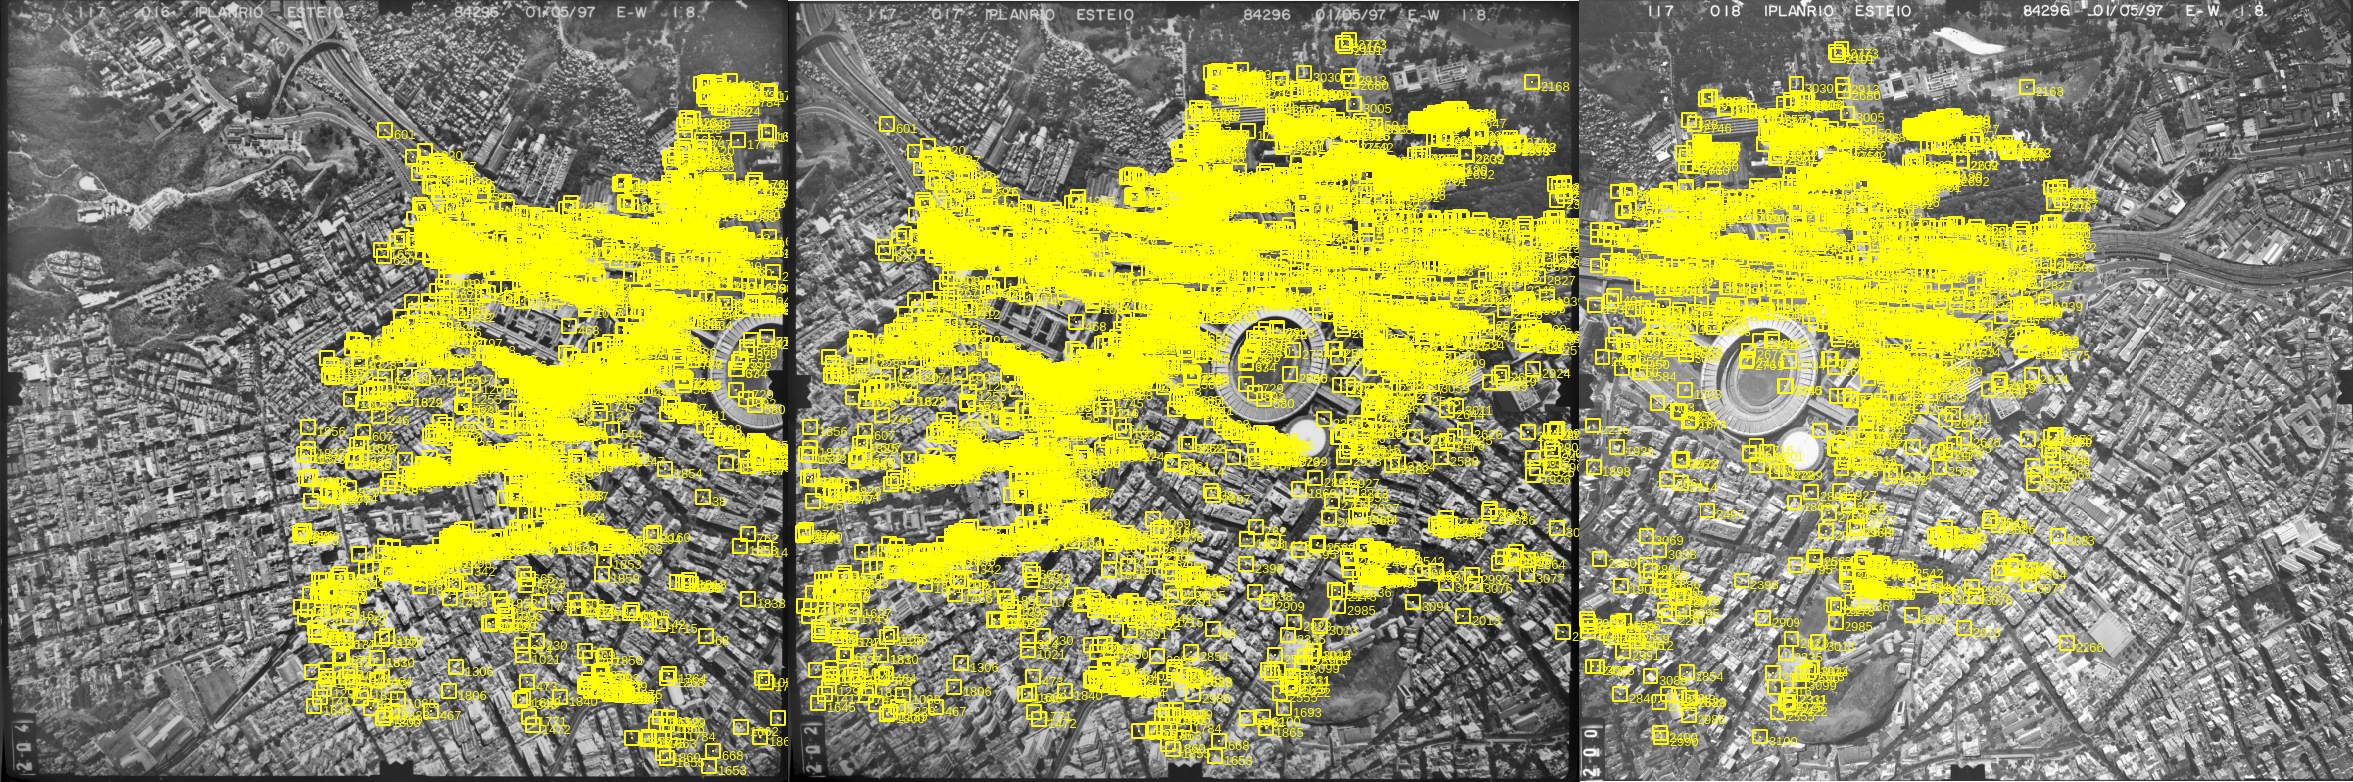
\includegraphics[width=1\hsize]{figuras/16_17_18_AKAZE.png}}}\hfill
  \subfloat[][]{\label{ORB}
    \fbox{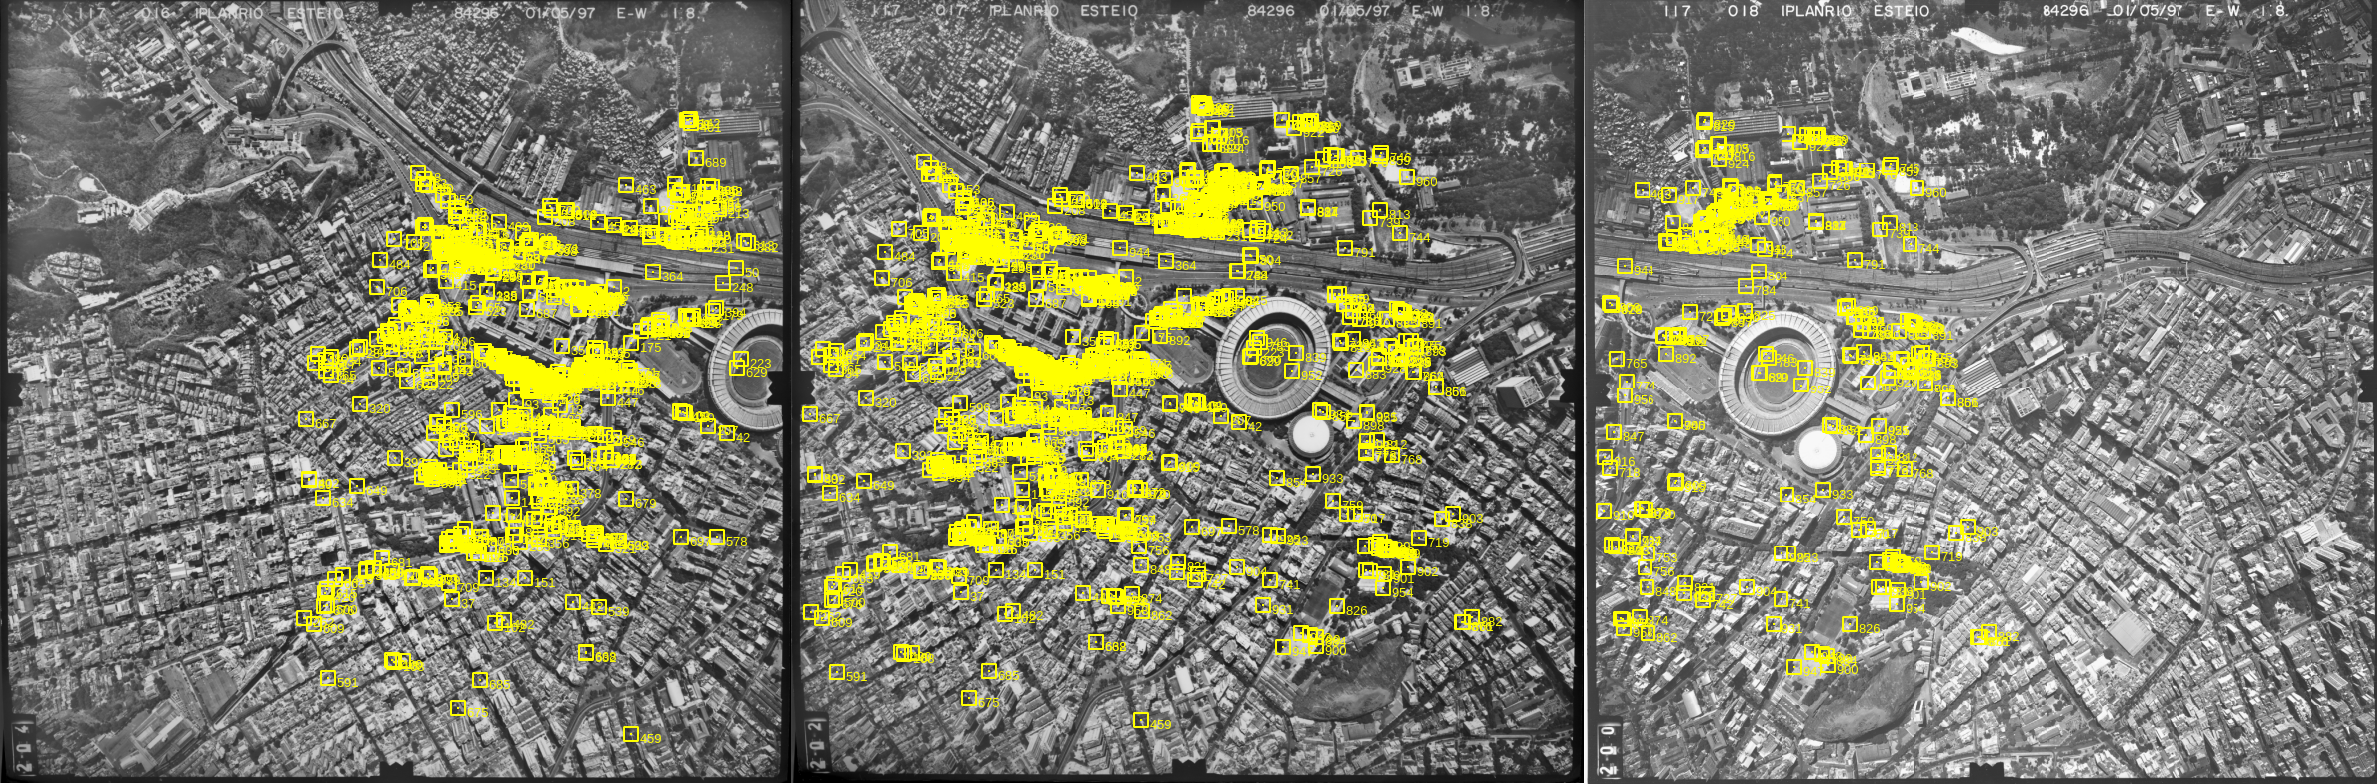
\includegraphics[width=1\hsize]{figuras/16_17_18_ORB.png}}}\hfill
  \subfloat[][]{\label{SIFT}
    \fbox{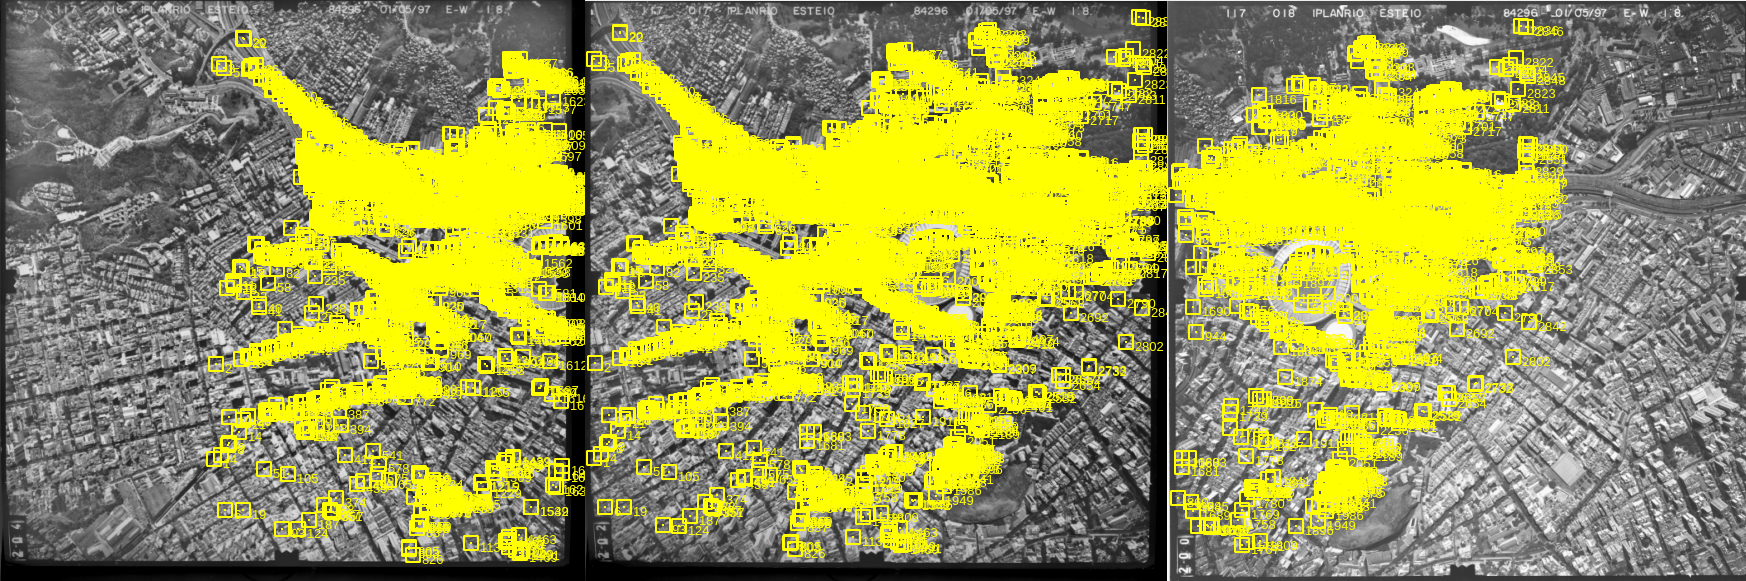
\includegraphics[width=1\hsize]{figuras/16_17_18_SIFT.png}}}\hfill
  \subfloat[][]{\label{SURF}
    \fbox{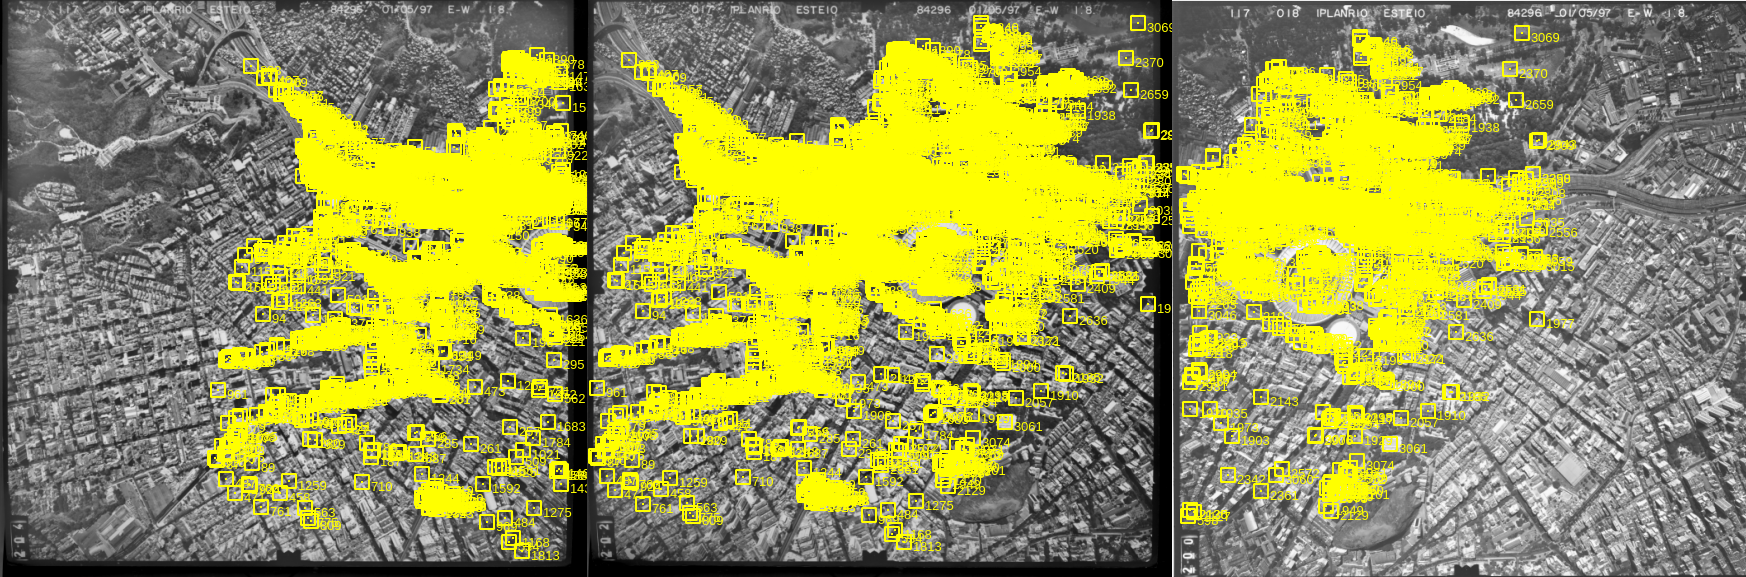
\includegraphics[width=1\hsize]{figuras/16_17_18_SURF.png}}}\hfill
  \legend{Resultados exibidos após inserção dos pontos no arquivo UERJ\_IO.epp, disponibilizado pelo Projeto E$-$Foto, que utiliza as imagens 16, 17 e 18 com:
          \subref{AKAZE} Resultado obtido com o método AKAZE;
          \subref{ORB} Resultado obtido com o método ORB;
          \subref{SIFT} Resultado obtido com o método SIFT; e
          \subref{SURF} Resultado obtido com o método SURF.}
  \source{O autor.}
\end{figure}

Para viabilizar a verificação da qualidade dos pontos de costura foram feitos recortes de tamanho regular na vizinhança das medidas nas imagens onde foram computados pela solução. Nos recortes o ponto medido corresponde ao centro e sua marcação foi omitida para não interferir na identificação dos pares. Ao todo, 20 pontos de costura em cada par foram isolados e encontram-se apresentados na Figura \ref{quality}. Em nenhum dos pares foi observado erro grosseiro, mas é possível notar que há variações como iluminação, deslocamento devido ao relevo ou de objetos moveis e desfoque. A rotação entre os recortes não é notada, pois há muito pouca rotação entre as imagens usadas para os testes.  

\begin{figure}[]{16cm}
  \caption{Seleção de recortes das imagens para verificação da qualidade} \label{quality}
    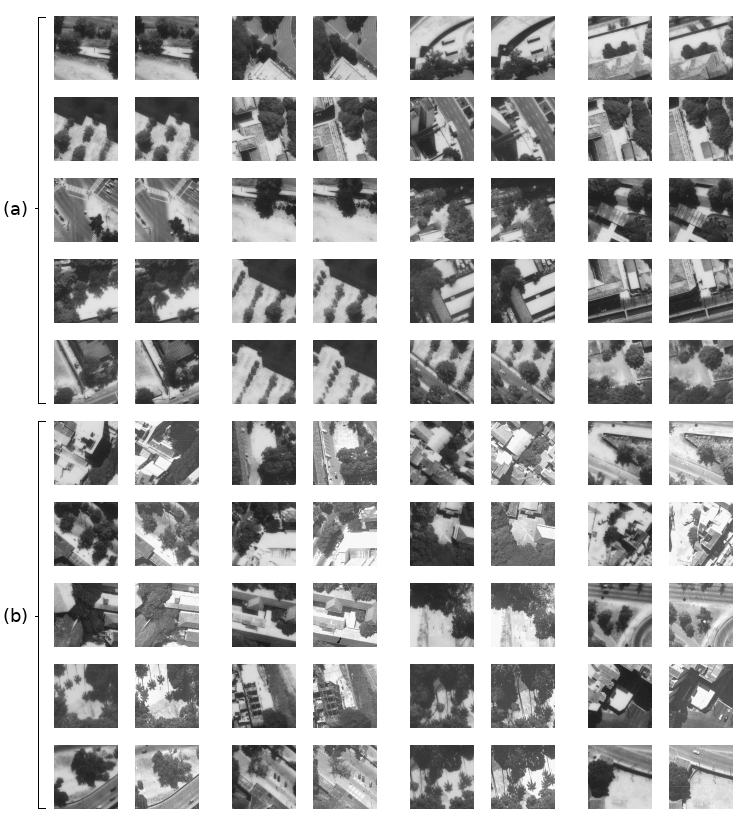
\includegraphics[width=1\hsize]{figuras/quality.png}
  \legend{Visualização de 20 pares de pontos selecionados nas imagens: (a) 16 e 17; e (b) 17 e 18.}
  \source{O autor.}
\end{figure}

Com intuito de atender aos critérios de restrição do número de respostas ou as regiões com respostas em diferentes fases do processamento foram estabelecidos parâmetros adicionais como o de filtragem baseada em regiões de interesse para detecção de pontos de gruber, outro para limitar o total de pontos chave usados para correlação e mais um para limitar \textit{inliers} usados para a solução final. Exemplos de padrões aplicáveis são oferecidos no Apêndice \ref{pattern}. O padrão 3-3-3, por exemplo, produz resultados como o apresentado na Figura \ref{pattern_res1}. Este padrão limita a área de procura em todas as imagens utilizadas, portanto deve ser criada com zelo, pois caso não exista regiões sobrepostas nos pares estes não trarão resultado.
A limitação do volume dos pontos de costura gerados pode ser visto na imagem \ref{pattern_res2}. Tal limite leva em consideração os melhores pontos, com menor RMSE, para gerar melhores resultados quando considerado a volumetria, por vezes excessiva, que os métodos poderiam retornar.

\begin{figure}[]{13cm}
  \caption{Imagem ilustrativa da resposta ao utilizar máscara.} \label{patterns_res}
  \subfloat[][]{\label{pattern_res1}
    \fbox{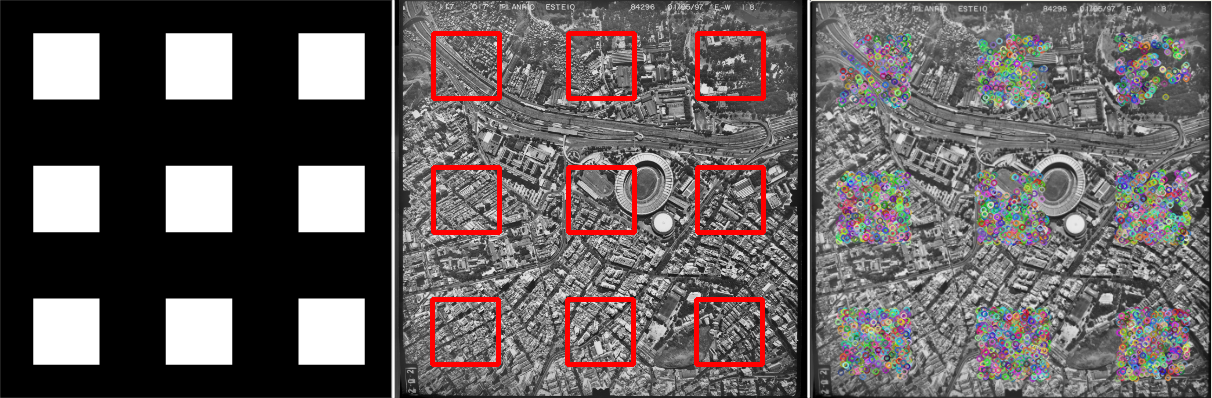
\includegraphics[width=1\hsize]{figuras/3_3_3_pattern.png}}}\hfill
  \subfloat[][]{\label{pattern_res2}
    \fbox{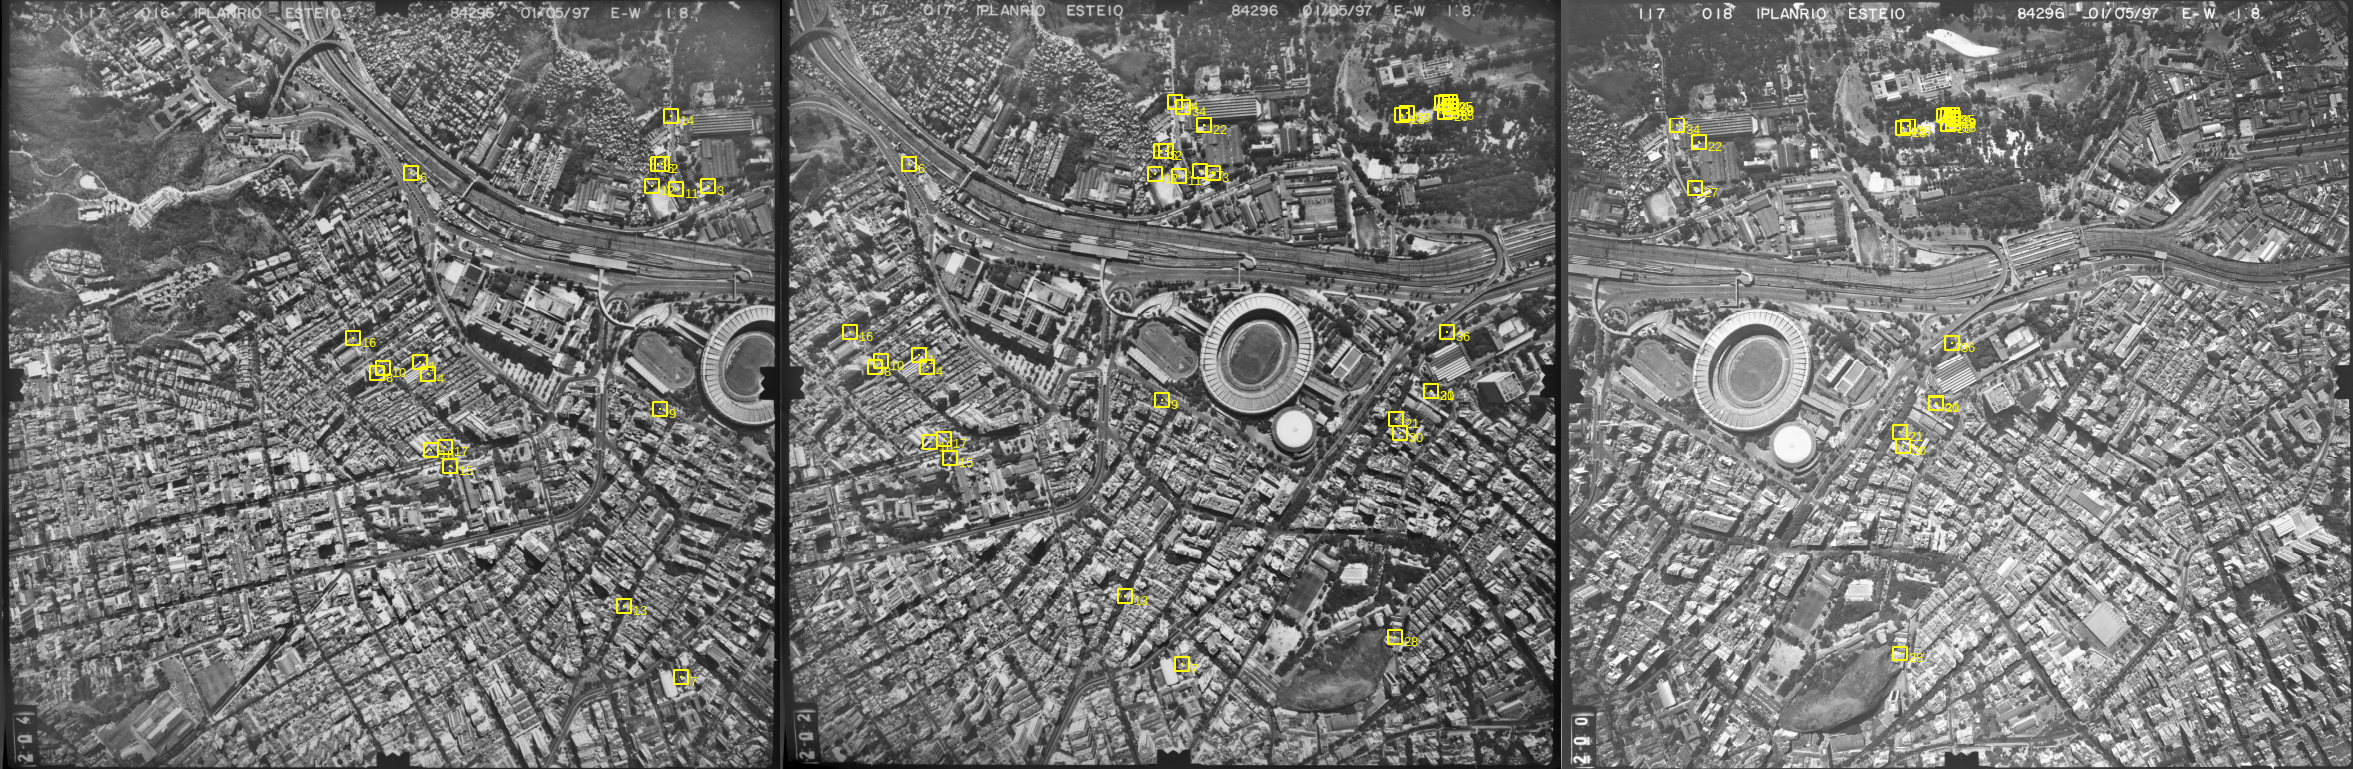
\includegraphics[width=1\hsize]{figuras/16_17_18_ORB_pattern_result.png}}}\\
  \legend{Imagens ilustrativas da resposta ao utilizar o padrão 3-3-3, com alternativas no apêndice \ref{pattern}, no método ORB com filtragem de pontos de costura.\\ \subref{pattern_res1} Imagens do padrão 3-3-3, onde este se aplicaria na imagem 17 e dos pontos chave detectados para esta imagem; e\\
  \subref{pattern_res2} Imagens 16, 17 e 18 com pontos de costura restritos às regiões de interesse e nas quantidades parametrizadas.}
  \source{O autor.}
\end{figure}

Cabe destacar que a limitação do volume de pontos chave detectados faz-se importante principalmente nas imagens de grandes resoluções, para evitar que o tempo de correlação cresça de forma descontrolada. Outra alternativa para o processamento destas imagens seria a redução das mesmas, por parâmetro da solução criado para este fim, pois entende-se que isto está relacionado a uma diminuição considerável no número máximo de pontos que podem ser detectados e que a solução proposta está pronta para lidar com a apresentação dos pontos de costura na escala da imagem original. 


\section{Impacto do uso de diferentes parâmetros}

Nesta seção são exibidas as principais variações que são introduzidas no resultado ao alterar os valores dos diferentes parâmetros, a fim de ilustrar como os valores de referência podem ser manipulados para atender a outras aplicações.

\subsection{Variação dos métodos de correlação}

Para discutir a diferença entre os métodos de correlação, que em nosso caso são o BFM e o FLANN, e o motivo que levou à escolha do algoritmo FLANN como parâmetro base a Figura \ref{GRAPH} exibe um gráfico que foi montado a partir dos resultados de tempo obtidos para ambos os métodos disponíveis. Adotou-se detecção e descrição pelo ORB, pois este sempre atende a quantidade de pontos chaves a serem extraídos, assim possibilitando a demonstração de escalabilidade do método de correlação. Foram adotadas 500, 1000, 2500, 5000, 7500, 10000 extrações, e plotadas as curvas para cada método de correlação representando o aumento do tempo de correlação em função do volume de pontos chave na entrada. 

\begin{figure}[]{16cm}
  \caption{Gráfico da diferença entre métodos de correlação BFM e FLANN.} \label{GRAPH}
  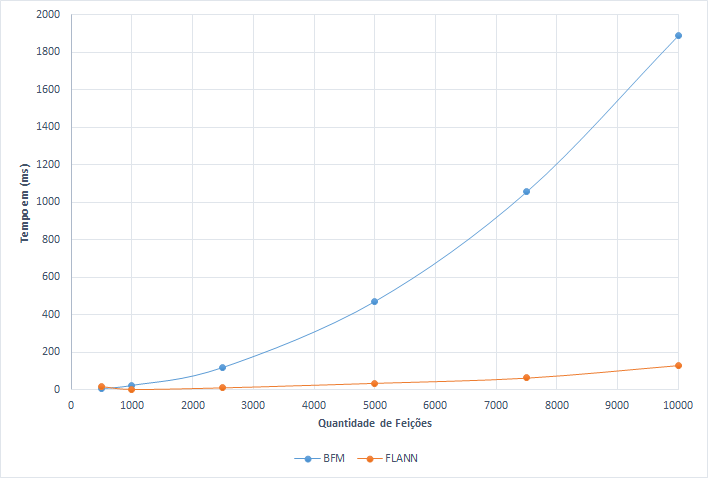
\includegraphics[width=\hsize]{figuras/Grafico.png}
  \legend{Eixo vertical demonstra o tempo em milissegundos, e o eixo horizontal a quantidade de pontos chaves nas imagens de cada par.}
  \source{O autor.}
\end{figure}

Pode-se captar no gráfico que o uso de força bruta não tem boa escalabilidade, pois o aumento de tempo para seu funcionamento se aproxima de um aumento exponencial, enquanto o aumento do método baseado em vizinho mais próximos aproximados é quase linear neste intervalo. Mesmo extrapolando o número de pontos extraídos, para 250 mil por exemplo, FLANN parece manter o comportamento quase linear, contudo neste intervalo seria impossível observar o ponto em que as curvas se cruzam. Deve ser ressaltado também que, quando a quantidade de pontos é muito baixa, inferior a 1000 no gráfico, este método tem tempo de execução pior que seu concorrente.

Apesar do desempenho, quando analisado o RMSE das mesmas soluções, mantido o total de pontos chave abaixo de 10000 pontos, o BFM retorna melhores correlatos devido principalmente à adoção de correlação cruzada, ou seja, atinge resíduos menores ao eliminar correlações que não são observáveis nos dois sentidos de análise (quando se compara uma imagem A com B e em seguida a imagem B com A). 

\subsection{Variação dos resíduos}

Nesta seção demonstra-se as alterações observáveis do resultado quando variado o resíduo máximo admitido nas soluções geométricas computadas para os pares processados. O tempo de processamento total no ajustamento das soluções geométricas dos pares, o RMSE resultante por par e o número dos pontos de costura na saída são apresentados na Tabela \ref{residuo}, onde foi utilizado exclusivamente o ORB como método de detecção e descrição.

A fim de alcançar melhores resultados foram escolhidos valores máximos de resíduo para análise dentro das recomendações da OpenCV\footnote{Mais informações podem ser encontradas na documentação do processo \textit{findHomography} em \url{https://docs.opencv.org/4.x/d9/d0c/group\_\_calib3d.html\#ga4abc2ece9fab9398f2e560d53c8c9780}}, exceto por um valor abaixo dos limites sugeridos para observar a viabilidade de manter resultados com restrições mais acentuadas.
Pode-se notar que mesmo com o resíduo máximo aumentado o RMSE pode não acompanhar esse aumento diretamente. Isso se dá por dois motivos: estamos apenas acrescentando poucos novos resíduos altos, que não passam a ser maioria no cálculo; e porque a solução continua sendo refinada (usando \textit{inliers} apenas se forem usados métodos robustos) com o método de Levenberg-Marquardt.
O custo de tempo diminui conforme o resíduo aumenta, isso se dá pois o processo de encontrar a matriz homográfica é um processo iterativo baseado em confiança. Portanto, quando este encontra muitas iterações com resíduo abaixo do solicitado, ele reduz o número de iterações restantes e acelera a entrega do resultado.

\begin{table}[]{15cm}
\centering
\caption{Resposta aos diferentes valores de resíduo máximo aplicáveis}
\label{residuo}
\begin{tabular}{c|cc|c|c|c}
\hline
\multirow{2}{*}{Resíduo} &
  \multicolumn{2}{c|}{RMSE} &
  \multirow{2}{*}{Média} &
  \multirow{2}{*}{\begin{tabular}[c]{@{}c@{}}Tempo\\  total\end{tabular}} &
  \multirow{2}{*}{\begin{tabular}[c]{@{}c@{}}Pontos de\\ costura\end{tabular}} \\ \cline{2-3}
    & \multicolumn{1}{c|}{16 x 17}  & 17 x 18  &          &         &      \\ \hline
0,5 & \multicolumn{1}{c|}{0,334696} & 0,33891  & 0,336803 & 68,0047 & 169  \\ \hline
1   & \multicolumn{1}{c|}{0,658826} & 0,648102 & 0,653464 & 68,5509 & 537  \\ \hline
2   & \multicolumn{1}{c|}{1,19721}  & 1,23801  & 1,21761  & 67,815  & 1467 \\ \hline
3   & \multicolumn{1}{c|}{1,83996}  & 1,69305  & 1,766505 & 45,6131 & 2295 \\ \hline
4   & \multicolumn{1}{c|}{2,18077}  & 2,13489  & 2,15783  & 23,2233 & 2697 \\ \hline
5   & \multicolumn{1}{c|}{2,39894}  & 2,46765  & 2,433295 & 15,3314 & 3025 \\ \hline
6   & \multicolumn{1}{c|}{2,79574}  & 2,88174  & 2,83874  & 10,8983 & 3374 \\ \hline
7   & \multicolumn{1}{c|}{2,9575}   & 3,14462  & 3,05106  & 9,0656  & 3690 \\ \hline
8   & \multicolumn{1}{c|}{3,09234}  & 3,33832  & 3,21533  & 8,54693 & 3856 \\ \hline
9   & \multicolumn{1}{c|}{3,22821}  & 3,51434  & 3,371275 & 9,17461 & 3972 \\ \hline
10  & \multicolumn{1}{c|}{3,24963}  & 3,68748  & 3,468555 & 7,52193 & 3771 \\ \hline
\end{tabular}
\legend{Resíduo: é valor escolhido ao executar o processo \textit{findHomography} na solução; RMSE: é a raiz quadrada do erro médio em cada par de imagens; Média: dos RMSE observados; Tempo total: da verificação geométrica; e Pontos de costura: gerados pela solução.}
\end{table}
